\documentclass[landscape]{tikzposter}
\geometry{paperwidth=36in,paperheight=48in}
\usepackage[english]{babel}
\usepackage{blindtext}
\usepackage{subfig}
\usepackage{listings}
\usepackage{adjustbox}
\usepackage{hyperref}
\title{\parbox{0.4\linewidth}{\centering Isosurface Extraction with \\ Cascading Transition Voxel Cells}}
\institute{Idaho State University, College of Science and Engineering}
\author{Jonathan Glines, with undergraduate advisor Dr. John Edwards}

\makeatletter
\def\TP@titlegraphictotitledistance{-9cm}
\settitle{ \vbox{
\@titlegraphic \hfill \\ [\TP@titlegraphictotitledistance]
\centering
\color{titlefgcolor} {\bfseries \Huge \sc \@title \par}
\vspace*{1em}
{\huge \@author \par} \vspace*{1em} {\LARGE \@institute}
}}
\makeatother

\titlegraphic{

\includegraphics[trim={2.5in 3in 3in 2.5in},scale=1.4]{isu-wordmark.pdf}
 \hfill
}

\usetheme{Simple} % See Section 5
\definecolor{bengalOrange}{cmyk}{0,0.65,1,0}
\definecolorstyle{BengalColorStyle} {
\definecolor{colorOne}{named}{white}
\definecolor{colorTwo}{named}{bengalOrange}
\definecolor{colorThree}{named}{black}
}{
% Background Colors
\colorlet{backgroundcolor}{colorOne}
\colorlet{framecolor}{black}
% Title Colors
\colorlet{titlefgcolor}{black}
\colorlet{titlebgcolor}{colorTwo}
% Block Colors
\colorlet{blocktitlebgcolor}{colorThree}
\colorlet{blocktitlefgcolor}{colorTwo}
\colorlet{blockbodybgcolor}{white}
\colorlet{blockbodyfgcolor}{black}
% Innerblock Colors
\colorlet{innerblocktitlebgcolor}{white}
\colorlet{innerblocktitlefgcolor}{black}
\colorlet{innerblockbodybgcolor}{colorThree!30!white}
\colorlet{innerblockbodyfgcolor}{black}
% Note colors
\colorlet{notefgcolor}{black}
\colorlet{notebgcolor}{colorTwo!50!white}
\colorlet{noteframecolor}{colorTwo}
}
\usecolorstyle{BengalColorStyle}

\usetitlestyle{Filled}
\begin{document}
\maketitle % See Section 4.1
\begin{columns}
\column{0.33}
\block{\Huge Isosurface Extraction}{
\input{isosurfaceExtraction.tex}
}
\begin{subcolumns} % See Section 4.4
\subcolumn{0.5} % See Section 4.4
\block{Original Marching Cubes}{
The original marching cubes algorithm as described by Lorensen and Cline 
}
\subcolumn{0.5}
\block{Dual Marching Cubes}{
The dual of the marching cubes is easiest to understand by looking at the
popular voxel game Minecraft.
}
\end{subcolumns}
\column{0.33}
\block{\Huge Isosurface Extraction Implementation}{
We set out to implement many of these isosurface extraction algorithms in an
easy-to-use library. The result is a C/C++ library we call \texttt{libmc}. The
goal of this library is to expose a simple and easy to use interface .

\texttt{libmc} is currently in the early stages of development. It is available
on github at the following url: \url{https://github.com/auntieNeo/libmc}
}
\newcommand{\examplesize}{3in}
\block{Example Output}{
\begin{minipage}[t]{\linewidth}
\begin{tikzfigure}[Original Marching Cubes]
\includegraphics[width=\examplesize,height=\examplesize]{../build/MC_SIMPLE_MARCHING_CUBES_cube_cd.png}
\end{tikzfigure}
\begin{tikzfigure}[Marching Cubes Patch]
\includegraphics[width=\examplesize,height=\examplesize]{../build/MC_PATCH_MARCHING_CUBES_cube_cd.png}
\end{tikzfigure}
\end{minipage}
\begin{adjustbox}{valign=t}
\begin{minipage}[t]{0.5\linewidth}
\begin{tikzfigure}[Cuberille]
\includegraphics[width=\examplesize,height=\examplesize]{../build/MC_CUBERILLE_cube_cd.png}
\end{tikzfigure}
\begin{tikzfigure}[Nielson's Dual Marching Cubes]
\includegraphics[width=\examplesize,height=\examplesize]{../build/MC_NIELSON_DUAL_cube_cd.png}
\end{tikzfigure}
\end{minipage}
\end{adjustbox}
}
\block{Example C++ Usage}{
\lstinputlisting[language=C]{example.c}
}
\column{0.33}
\block{\Huge Cascading Transition Voxel Cells}{Blocktext}
\begin{subcolumns}
\subcolumn{0.5}
\block{Generalizing the Transvoxel Algorithm}{
The Transvoxel algorithm, as described by Lengyel in FIXME,
\\ \\
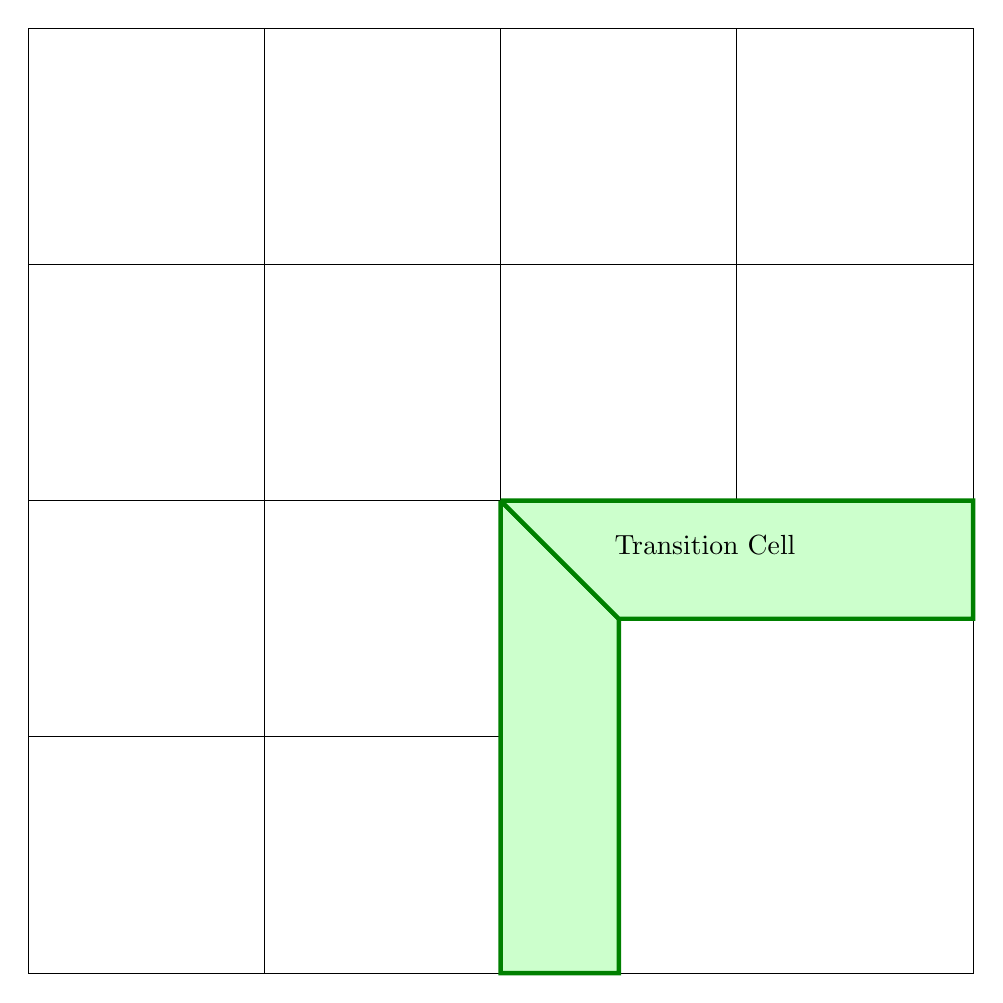
\begin{tikzpicture}[scale=3]
  \draw (0, 0) rectangle (1, 1);
  \draw (1, 0) rectangle (2, 1);
  \draw (0, 1) rectangle (1, 2);
  \draw (1, 1) rectangle (2, 2);

  \draw (2, 2) rectangle (3, 3);
  \draw (3, 2) rectangle (4, 3);
  \draw (2, 3) rectangle (3, 4);
  \draw (3, 3) rectangle (4, 4);

  \draw (0, 2) rectangle (1, 3);
  \draw (1, 2) rectangle (2, 3);
  \draw (0, 3) rectangle (1, 4);
  \draw (1, 3) rectangle (2, 4);

  \draw (2.5, 0) rectangle (4, 1.5);

  \begin{scope}[ultra thick]
    \filldraw[fill=green!20!white, draw=green!50!black] (2, 2) -- (2, 0) -- (2.5, 0) -- (2.5, 1.5) -- (2, 2);
    \filldraw[fill=green!20!white, draw=green!50!black] (2, 2) -- (4, 2) -- (4, 1.5) -- (2.5, 1.5) -- (2, 2) node [below=1.6em, right=3.7em] {Transition Cell};
  \end{scope}
\end{tikzpicture} \\ \\

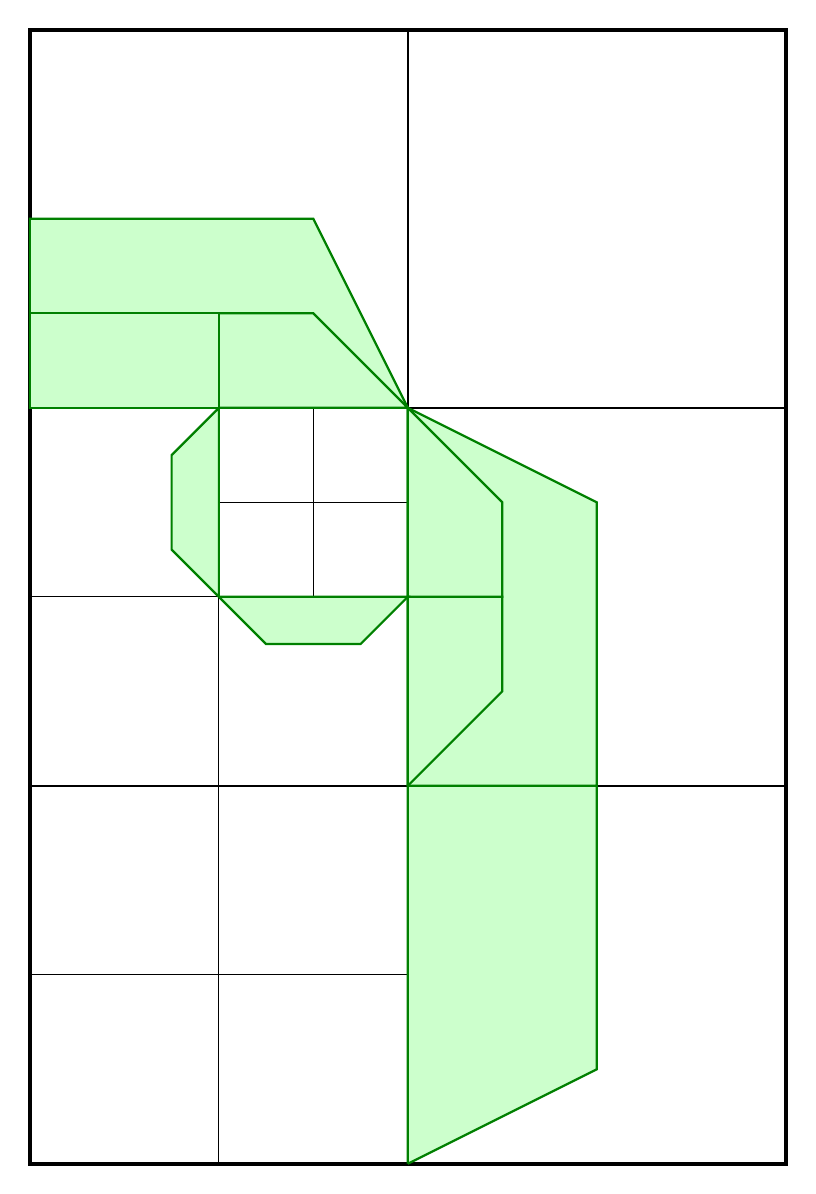
\begin{tikzpicture}[scale=1.2]
  % Draw a border around the quadtree figure
  \begin{scope}[ultra thick]
    \draw (0, 0) rectangle (8, 12);
  \end{scope}
  % Draw the quadtree nodes at three levels
  \begin{scope}[thick]
    \draw (0, 0) rectangle (4, 4);
    \draw (4, 0) rectangle (8, 4);
    \draw (0, 4) rectangle (4, 8);
    \draw (4, 4) rectangle (8, 8);
    \draw (0, 8) rectangle (4, 12);
    \draw (4, 8) rectangle (8, 12);
  \end{scope}
  \begin{scope}
    \draw (0, 0) rectangle (2, 2);
    \draw (2, 0) rectangle (4, 2);
    \draw (0, 2) rectangle (2, 4);
    \draw (2, 2) rectangle (4, 4);

    \draw (0, 4) rectangle (2, 6);
    \draw (2, 4) rectangle (4, 6);
    \draw (0, 6) rectangle (2, 8);
    \draw (2, 6) rectangle (4, 8);
  \end{scope}
  \begin{scope}[very thin]
    \draw (2, 6) rectangle (3, 7);
    \draw (3, 6) rectangle (4, 7);
    \draw (2, 7) rectangle (3, 8);
    \draw (3, 7) rectangle (4, 8);
  \end{scope}
  % Draw the transition cells, being careful to draw the larger ones first
  \begin{scope}[fill=green!20!white, draw=green!50!black, thick]
    % Large transitions
    \filldraw (4, 0) -- (6, 1) -- (6, 4) -- (4, 4) -- (4, 0);
    \filldraw (4, 4) -- (6, 4) -- (6, 7) -- (4, 8) -- (4, 4);
    \filldraw (4, 8) -- (3, 10) -- (0, 10) -- (0, 8) -- (4, 8);
    % Small transitions
    \filldraw (4, 4) -- (5, 5) -- (5, 6) -- (4, 6) -- (4, 4);
    \filldraw (4, 6) -- (5, 6) -- (5, 7) -- (4, 8) -- (4, 6);
    \filldraw (4, 8) -- (3, 9) -- (2, 9) -- (2, 8) -- (4, 8);
    \filldraw (0, 8) -- (2, 8) -- (2, 9) -- (0, 9) -- (0, 8);
    % Smallest transitions
    \filldraw (2, 6) -- (2.5, 5.5) -- (3.5, 5.5) -- (4, 6) -- (2, 6);
    \filldraw (2, 6) -- (1.5, 6.5) -- (1.5, 7.5) -- (2, 8) -- (2, 6);
  \end{scope}
\end{tikzpicture}
}
\subcolumn{0.5}
\block{42 Regular Cell Cases}{Blocktext}
\block{73 Transition Cell Cases}{
%  MC_TRANSVOXEL_CANONICAL_TRANSITION_CELL_0 = 0x000,
%  MC_TRANSVOXEL_CANONICAL_TRANSITION_CELL_1 = 0x001,
%  MC_TRANSVOXEL_CANONICAL_TRANSITION_CELL_2 = 0x002,
%  MC_TRANSVOXEL_CANONICAL_TRANSITION_CELL_3 = 0x003,
%  MC_TRANSVOXEL_CANONICAL_TRANSITION_CELL_4 = 0x005,
%  MC_TRANSVOXEL_CANONICAL_TRANSITION_CELL_5 = 0x007,
%  MC_TRANSVOXEL_CANONICAL_TRANSITION_CELL_6 = 0x00a,
%  MC_TRANSVOXEL_CANONICAL_TRANSITION_CELL_7 = 0x00b,
%  MC_TRANSVOXEL_CANONICAL_TRANSITION_CELL_8 = 0x00c,
%  MC_TRANSVOXEL_CANONICAL_TRANSITION_CELL_9 = 0x00d,
%  MC_TRANSVOXEL_CANONICAL_TRANSITION_CELL_10 = 0x00e,
%  MC_TRANSVOXEL_CANONICAL_TRANSITION_CELL_11 = 0x00f,
%  MC_TRANSVOXEL_CANONICAL_TRANSITION_CELL_12 = 0x010,
%  MC_TRANSVOXEL_CANONICAL_TRANSITION_CELL_13 = 0x011,
%  MC_TRANSVOXEL_CANONICAL_TRANSITION_CELL_14 = 0x012,
%  MC_TRANSVOXEL_CANONICAL_TRANSITION_CELL_15 = 0x013,
%  MC_TRANSVOXEL_CANONICAL_TRANSITION_CELL_16 = 0x015,
%  MC_TRANSVOXEL_CANONICAL_TRANSITION_CELL_17 = 0x017,
%  MC_TRANSVOXEL_CANONICAL_TRANSITION_CELL_18 = 0x01a,
%  MC_TRANSVOXEL_CANONICAL_TRANSITION_CELL_19 = 0x01b,
%  MC_TRANSVOXEL_CANONICAL_TRANSITION_CELL_20 = 0x01c,
%  MC_TRANSVOXEL_CANONICAL_TRANSITION_CELL_21 = 0x01d,
%  MC_TRANSVOXEL_CANONICAL_TRANSITION_CELL_22 = 0x01e,
%  MC_TRANSVOXEL_CANONICAL_TRANSITION_CELL_23 = 0x028,
%  MC_TRANSVOXEL_CANONICAL_TRANSITION_CELL_24 = 0x029,
%  MC_TRANSVOXEL_CANONICAL_TRANSITION_CELL_25 = 0x02a,
%  MC_TRANSVOXEL_CANONICAL_TRANSITION_CELL_26 = 0x02b,
%  MC_TRANSVOXEL_CANONICAL_TRANSITION_CELL_27 = 0x02d,
%  MC_TRANSVOXEL_CANONICAL_TRANSITION_CELL_28 = 0x038,
%  MC_TRANSVOXEL_CANONICAL_TRANSITION_CELL_29 = 0x039,
%  MC_TRANSVOXEL_CANONICAL_TRANSITION_CELL_30 = 0x03a,
%  MC_TRANSVOXEL_CANONICAL_TRANSITION_CELL_31 = 0x03b,
%  MC_TRANSVOXEL_CANONICAL_TRANSITION_CELL_32 = 0x03d,
%  MC_TRANSVOXEL_CANONICAL_TRANSITION_CELL_33 = 0x044,
%  MC_TRANSVOXEL_CANONICAL_TRANSITION_CELL_34 = 0x045,
%  MC_TRANSVOXEL_CANONICAL_TRANSITION_CELL_35 = 0x046,
%  MC_TRANSVOXEL_CANONICAL_TRANSITION_CELL_36 = 0x04e,
%  MC_TRANSVOXEL_CANONICAL_TRANSITION_CELL_37 = 0x054,
%  MC_TRANSVOXEL_CANONICAL_TRANSITION_CELL_38 = 0x055,
%  MC_TRANSVOXEL_CANONICAL_TRANSITION_CELL_39 = 0x056,
%  MC_TRANSVOXEL_CANONICAL_TRANSITION_CELL_40 = 0x057,
%  MC_TRANSVOXEL_CANONICAL_TRANSITION_CELL_41 = 0x05e,
%  MC_TRANSVOXEL_CANONICAL_TRANSITION_CELL_42 = 0x061,
%  MC_TRANSVOXEL_CANONICAL_TRANSITION_CELL_43 = 0x062,
%  MC_TRANSVOXEL_CANONICAL_TRANSITION_CELL_44 = 0x063,
%  MC_TRANSVOXEL_CANONICAL_TRANSITION_CELL_45 = 0x065,
%  MC_TRANSVOXEL_CANONICAL_TRANSITION_CELL_46 = 0x066,
%  MC_TRANSVOXEL_CANONICAL_TRANSITION_CELL_47 = 0x06a,
%  MC_TRANSVOXEL_CANONICAL_TRANSITION_CELL_48 = 0x06b,
%  MC_TRANSVOXEL_CANONICAL_TRANSITION_CELL_49 = 0x06c,
%  MC_TRANSVOXEL_CANONICAL_TRANSITION_CELL_50 = 0x06e,
%  MC_TRANSVOXEL_CANONICAL_TRANSITION_CELL_51 = 0x071,
%  MC_TRANSVOXEL_CANONICAL_TRANSITION_CELL_52 = 0x072,
%  MC_TRANSVOXEL_CANONICAL_TRANSITION_CELL_53 = 0x073,
%  MC_TRANSVOXEL_CANONICAL_TRANSITION_CELL_54 = 0x075,
%  MC_TRANSVOXEL_CANONICAL_TRANSITION_CELL_55 = 0x076,
%  MC_TRANSVOXEL_CANONICAL_TRANSITION_CELL_56 = 0x077,
%  MC_TRANSVOXEL_CANONICAL_TRANSITION_CELL_57 = 0x07c,
%  MC_TRANSVOXEL_CANONICAL_TRANSITION_CELL_58 = 0x07e,
%  MC_TRANSVOXEL_CANONICAL_TRANSITION_CELL_59 = 0x0aa,
%  MC_TRANSVOXEL_CANONICAL_TRANSITION_CELL_60 = 0x0ab,
%  MC_TRANSVOXEL_CANONICAL_TRANSITION_CELL_61 = 0x0ad,
%  MC_TRANSVOXEL_CANONICAL_TRANSITION_CELL_62 = 0x0af,
%  MC_TRANSVOXEL_CANONICAL_TRANSITION_CELL_63 = 0x0ba,
%  MC_TRANSVOXEL_CANONICAL_TRANSITION_CELL_64 = 0x0e5,
%  MC_TRANSVOXEL_CANONICAL_TRANSITION_CELL_65 = 0x0e7,
%  MC_TRANSVOXEL_CANONICAL_TRANSITION_CELL_66 = 0x0ee,
%  MC_TRANSVOXEL_CANONICAL_TRANSITION_CELL_67 = 0x0ef,
%  MC_TRANSVOXEL_CANONICAL_TRANSITION_CELL_68 = 0x0f5,
%  MC_TRANSVOXEL_CANONICAL_TRANSITION_CELL_69 = 0x0fe,
%  MC_TRANSVOXEL_CANONICAL_TRANSITION_CELL_70 = 0x155,
%  MC_TRANSVOXEL_CANONICAL_TRANSITION_CELL_71 = 0x157,
%  MC_TRANSVOXEL_CANONICAL_TRANSITION_CELL_72 = 0x15f,
\newcommand{\transcellsize}{1in}
\def\transcellcolumns{
{"000", "00a", "010", "01a", "029", "03a", "04e", "061", "06b", "075", "0ab", "0ee", "15f"},
{"001", "00b", "011", "01b", "02a", "03b", "054", "062", "06c", "076", "0ad", "0ef"},
{"002", "00c", "012", "01c", "02b", "03d", "055", "063", "06e", "077", "0af", "0f5"},
{"003", "00d", "013", "01d", "02d", "044", "056", "065", "071", "07c", "0ba", "0fe"},
{"005", "00e", "015", "01e", "038", "045", "057", "066", "072", "07e", "0e5", "155"},
{"007", "00f", "017", "028", "039", "046", "05e", "06a", "073", "0aa", "0e7", "157"}}
\foreach \column in \transcellcolumns
{
  \begin{adjustbox}{valign=t}
  \begin{minipage}[t]{0.15\linewidth}
  \foreach \cell in \column
  {
    \begin{tikzfigure}
    \includegraphics[width=\transcellsize,height=\transcellsize]{../build/MC_TRANSVOXEL_transition_cell_0x\cell.png}
    \end{tikzfigure}
  }
  \end{minipage}
  \end{adjustbox}
}
%\begin{minipage}[t]{0.1666\linewidth}
%\begin{tikzfigure}
%\includegraphics[width=1in,height=1in]{../build/MC_TRANSVOXEL_transition_cell_0x001.png}
%\end{tikzfigure}
%\end{minipage}
%\begin{adjustbox}{valign=t}
%\begin{minipage}[t]{0.5\linewidth}
%\begin{tikzfigure}[Cuberille]
%\includegraphics[width=4in,height=4in]{../build/MC_CUBERILLE_cube_cd.png}
%\end{tikzfigure}
%\begin{tikzfigure}[Nielson's Dual Marching Cubes]
%\includegraphics[width=4in,height=4in]{../build/MC_NIELSON_DUAL_cube_cd.png}
%\end{tikzfigure}
%\end{minipage}
%\end{adjustbox}

}
\end{subcolumns}
\end{columns}
\end{document}
